%%Berichtvorlage für EDBV WS 2014/2015

\documentclass[paper=A4, deutsch]{scrartcl}
\usepackage[ngerman]{babel}
\usepackage[utf8]{inputenc}
\usepackage{algorithmic}
\usepackage{algorithm}
\usepackage{graphicx}
\usepackage{amsmath,amssymb}
\usepackage{subcaption}
\captionsetup{compatibility=false}
\usepackage{multirow}
\usepackage{color}
\usepackage[]{geometry}
\graphicspath{ {./images/} }
\begin{document}


%%------------------------------------------------------
%% Ab hier tragt ihr eure Daten und Ergebnisse ein:
%%------------------------------------------------------

\title{nine-mans-morris} %%Projekttitel hier eintragen

\subtitle{EDBV WS 2018/2019: AG\_C3} %%statt XX Arbeitsgruppenbezeichnung hier eintragen (zB.: A1)


%%Namen und Matrikelnummern der Gruppenmitglieder hier eintragen
\author{Tobias Batik (11701221)\\
Bougouma Fall (01427956)\\
Yannic Ellhotka (11776168)\\
Lisalotte Tscherteu (0271430)\\
Simon Wesp (11709457)
}



%%------------------------------------------------------

\maketitle


%%------------------------------------------------------
\section{Gewählte Problemstellung}

\subsection{Ziel}
Bildserie eines Mühlespieles einlesen. Den aktuellen Spielstand erkennen und überprüfen ob das Spiel regelkonform gespielt wurde.  
\subsection{Eingabe}
Folge von Farbbildern des Spielbrettes. 


\subsection{Ausgabe}
Aktueller Spielstand in der Konsole. \\
Alle eingelesen Spielzüge und deren Spielstand als Textdatei. \\
Kontrolle ob ein Spiel regelkonform gespielt wurde. 
\subsection{Voraussetzungen und Bedingungen}
Bilder müssen annähernd in Volgelperspektive aufgenommen werden (+-30 Grad). \\
Das Spielbrett muss die in der Grafik dargestellten relativen Maßeinheiten erfüllen (siehe Abbildung 1) . 
Der Hintergrund der Spielfelder muss ausreichend Kontrast zu den weißen sowie schwarzen Spielsteinen aufweisen. \\
Die verwendeten Spielsteine haben eine durchmesser von Breite des Spielfelder * 0.08.\\
Steine müssen eindeutig auf den vorgesehen Punkten liegen.\\
Die Ecken des Spielfeldes und die Spielsteine dürfen nicht durch andere Gegestände verdeckt werden.\\
Kein anderer runder Gegenstand mit dem selben Radius wie die Spielsteine, darf auf den Spielfeld liegen. 
\begin{figure}[ht]
	\centering
		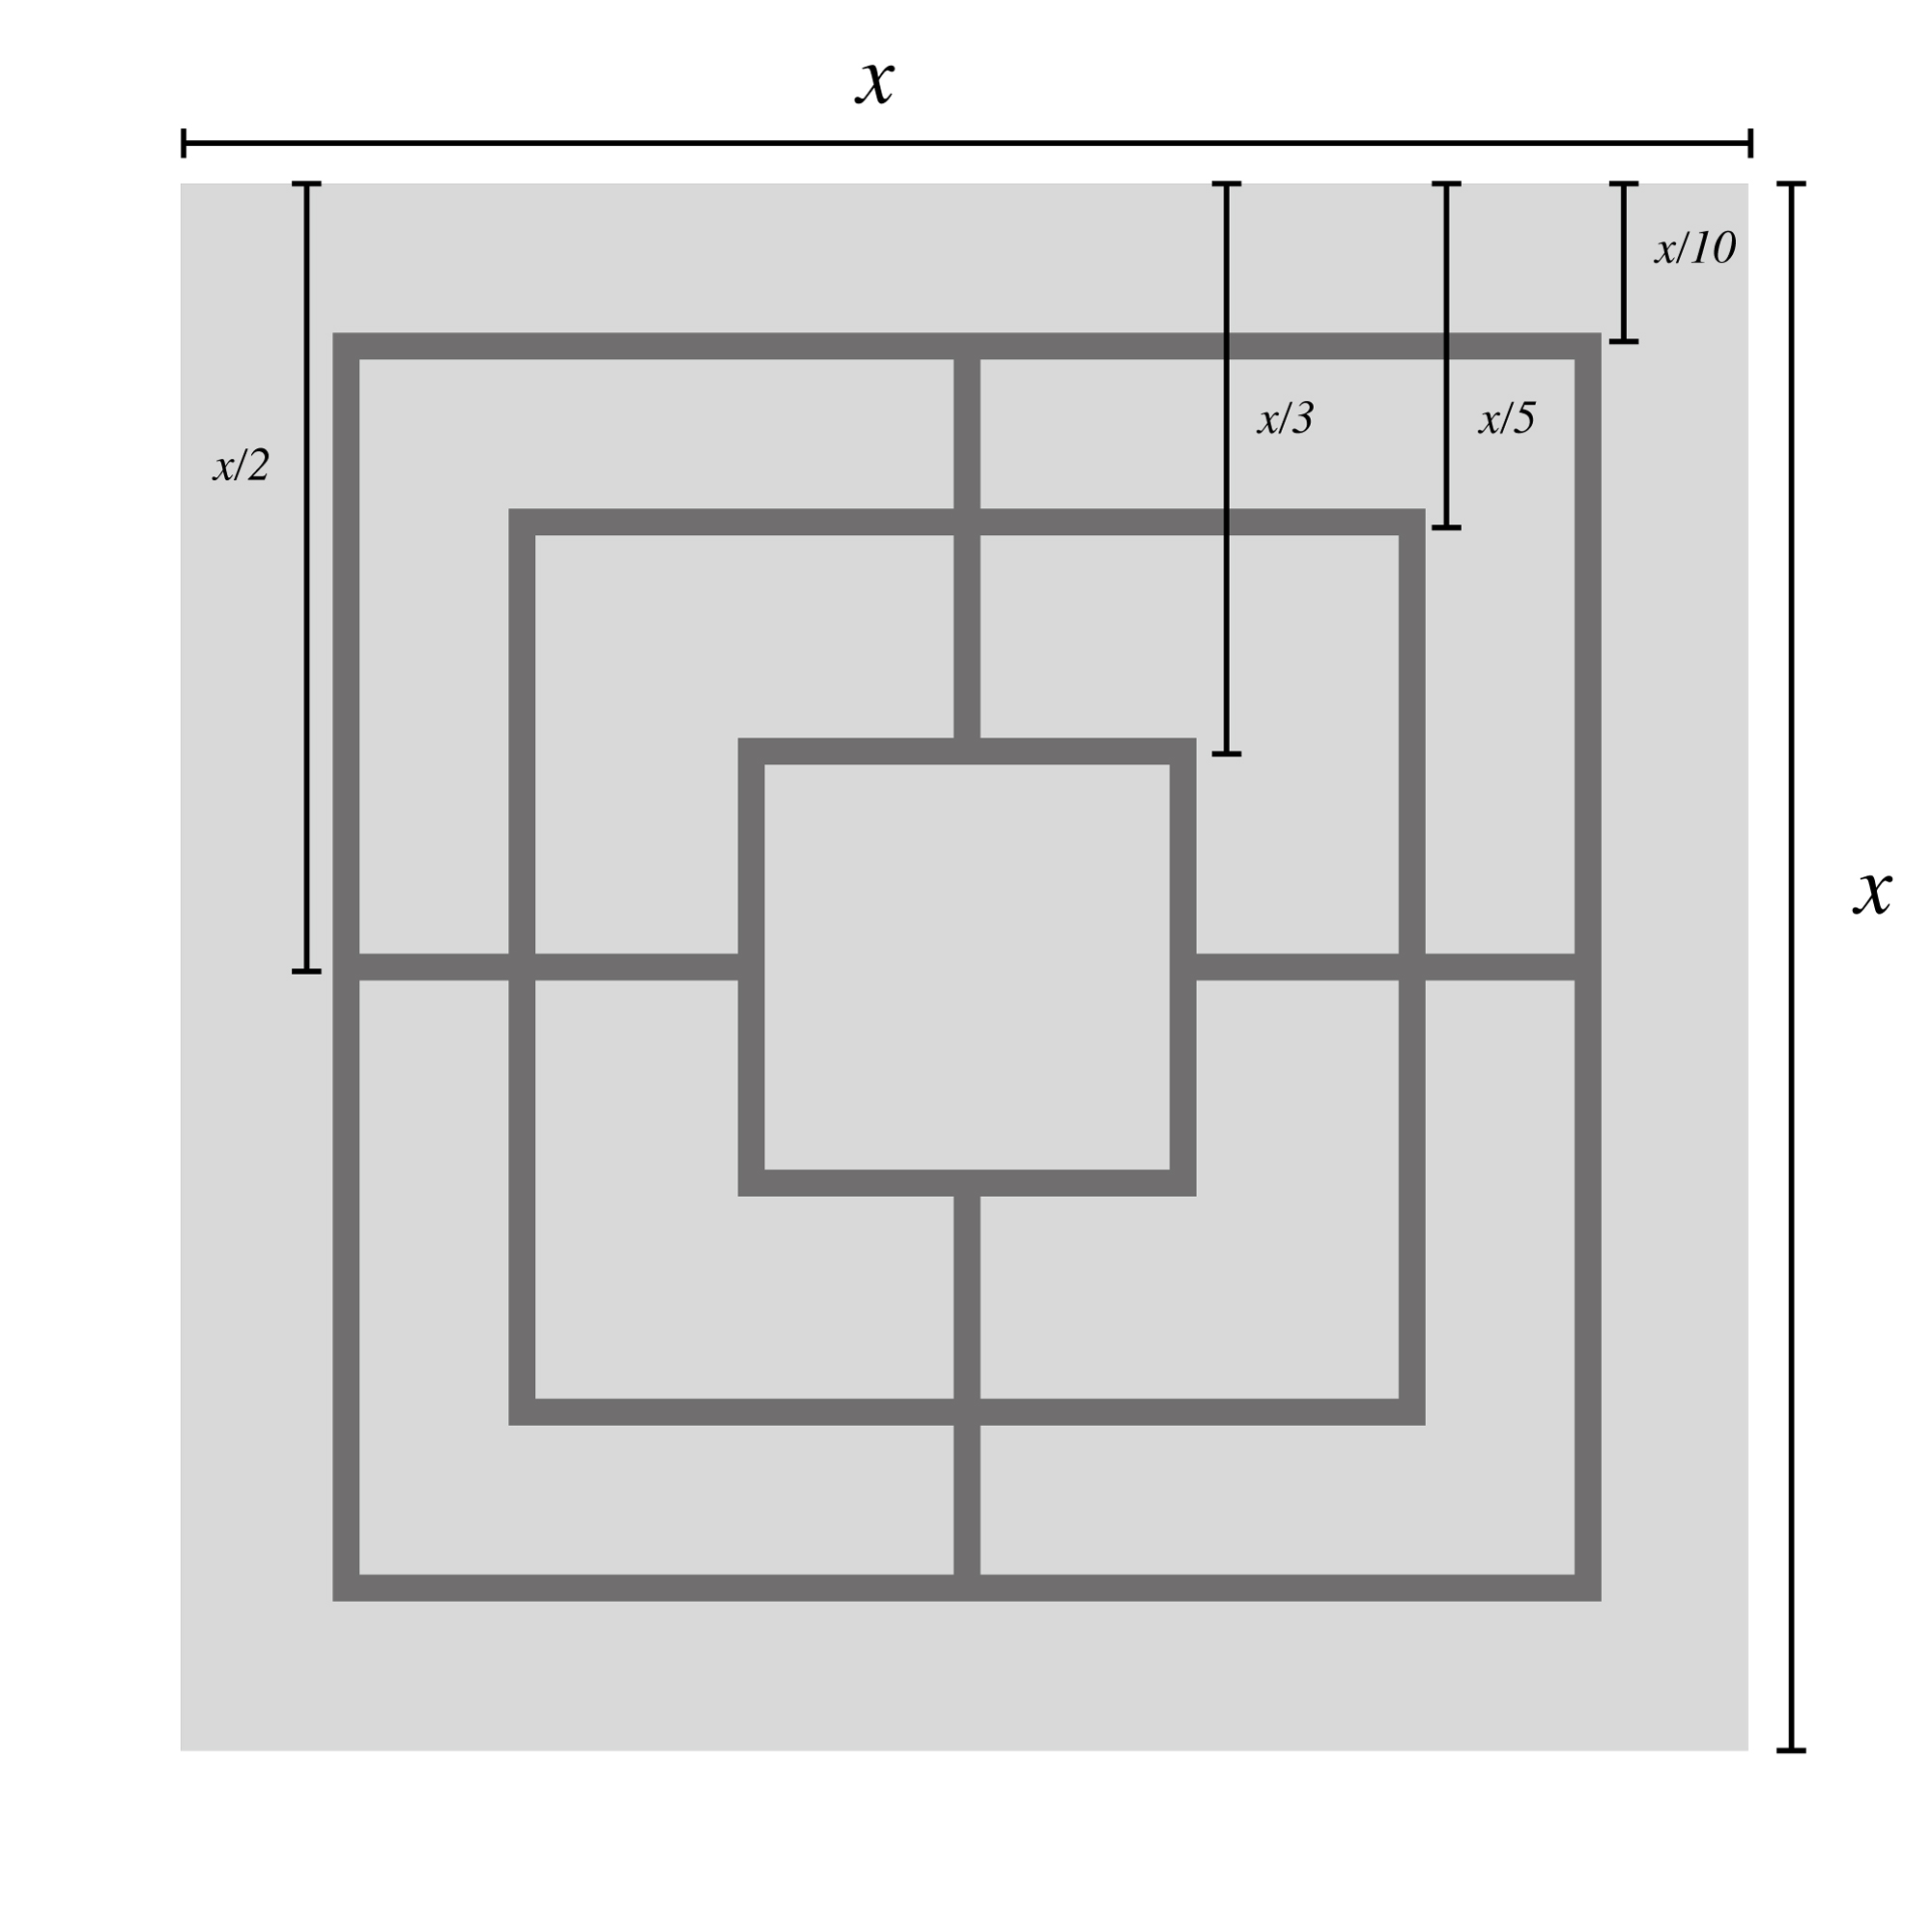
\includegraphics[width=8cm]{Spielbrett_relativeDimensionen_grafik.jpg}\\
	\caption[Relative Spielfelddimensionen]{Relative Spielfelddimensionen.}
	\label{fig:nettop}
\end{figure}



\subsection{Methodik}
1.  Threshold\\
\hspace*{1em} a. Input: rgb Bild des Spielfeldes\\
\hspace*{1em} b. Output: Eckpunkte des Spielfelder, Binärbild\\
2. Geometrische Transformation\\
\hspace*{1em} a. Input: rgb Bild des Spielfeldes und Koordinaten der Eckpunkte des Spielfeldes\\
\hspace*{1em} b. Output: entzerrtes 500 x 500 Pixel rgb Bild\\
3. Canny\\
\hspace*{1em} a. Input: entzerrtes 500 x 500 Pixel rgb Bild\\
\hspace*{1em} b. Output: Kantenbild \\
4. Hough-Transformation \\
\hspace*{1em} a. Input: Kanten-Bild des entzerrten Spielfeldes\\
\hspace*{1em} b. Output: Koordinaten der Mittelpunkte der Spielsteine \\
5. Spielstand erkennung \\
\hspace*{1em} a. Input: Koordinaten der Mittelpunkte der Spielsteine und rgb Bild des entzerrten Spielfeldes\\
\hspace*{1em} b. Output: 3x3x3 Array das den aktuellen Spielstand repräsentiert \\
6. Gültigkeit des Spielzuges\\
\hspace*{1em} a. Input: Voriger und aktueller Spielstand \\
\hspace*{1em} b. Output: Hinweis falls der Zug ungültig war

\subsection{Evaluierungsfragen}
1. Wird das Spielfeld richtig eingelesen?\\
%2. Wird ein gültiger Spielzug vorhergesagt?\\
2. Wird ein gültiges Spiel als solches erkannt?\\
\subsection{Zeitplan}

\begin{table}[h!]
	\centering
	\begin{tabular}{|c|c|c|c|c|}
		\hline
		Meilenstein & \multicolumn{2}{c|}{abgeschlossen am} & \multicolumn{2}{c|}{Arbeitsaufwand in h}\\
		\cline{2-5}
		 & geplant & tatsächlich & geplant & tatsächlich\\
		\hline
				Prototype, prof of konzept & 14.11 & 28.11 & X & 15\\
		\hline
				Datenbank 1 aufbauen & 1.12 & 26.11 & 10 & 10\\
		\hline
				Framework &15.10 &2.10 & X & 10\\
		\hline	
				Threshold und Eckenerkennung & 15.11 & 21.11 & 30 &35\\
		\hline	
				Geometrische Transformation & 29.11 & 5.12 & 70 &60\\
		\hline	
				Canny Kantenerkennung & 12.12 & 16.12 & 25 & 35\\
		\hline	
				Hough Kreiserkennung & 30.12 & 22.12 & 30 & 35\\
		\hline	
				Spielstanderkennung & 24.12 & 28.12 & 25 & 25\\
		\hline	
				Analyse des Spielzüge & 15.12 & 2.1 &20 &30\\
		\hline	
				Datenbank 2 aufbauen & X & 4.1 & X & 10\\
		\hline
				textueller Output & 28.12 &  3.1 & 10 & 10 \\
		\hline 
				Analyse \& Evaluierung & X & 6.1 & X & 12\\
		\hline
				Bericht & 6.1 & 6.1 & 40 & 45\\
		\hline
	\end{tabular}
\end{table}
%%------------------------------------------------------

%%------------------------------------------------------
\section{Arbeitsteilung}
\begin{center}
  \begin{tabular}{ |l | c | }
    \hline
  Name & Tätigkeiten\\
    \hline
			Tobias Batik & Matlab-Funktionen: hough, findStein; Bericht Abschnitt: 3.5, 4.5, 5.2.1, 5.3.Hough, 5.3.findstein,6\\
		\hline
			Bougouma Fall & Matlab-Funktionen: isLegit, getPhase, countOccurences, checkForMill; Bericht Abschnitt 3.6, 4.7, 5.2.2\\
		\hline
			Yannic Ellhotka & Matlab-Funktion: threshold, canny, GT; Bericht Abschnitt 3.1, 3.2, 4.2, 4.3, 4.4, 5.1\\
		\hline
			Lisalotte Tscherteu & Matlab-Funktion: hough, findStein; Bericht Abschnitt 4.6, Plakat\\
		\hline
			Simon Wesp & Matlab-Funktion: threshold, canny, GT; Bericht Abschnitt 3.1, 3.2, 4.2, 4.3, 4.4,6\\
		\hline
  \end{tabular}
\end{center}

%%------------------------------------------------------

%%------------------------------------------------------
\section{Methodik}

\subsection{Threshold und Eckenerkennung}
Beim Thresholding werden die Ecken des Spielfeldes aus dem Bild gesucht. Dafür müssen die Pixel, die weiß sind und die kleinsten/größten Koordinaten haben, herausgefunden werden. Es gibt aber immer wieder einzelne Ausßreisser im Bild - das kann von ISO-Noise, toten Pixeln am Kamerasensor oder Ähnlichem kommen. Deswegen wird vor der Eckenerkennung mit einem quadratischen Element über das Bild erodiert. So werden kleine Unregelmäßigkeiten ausgebügelt und das Ergebnis genauer. Der Threshold selbst dient dazul, das helle Spielfeld vom Hintergrund abzuheben - ist er richtig gewählt, ist es einfach, die ersten/letzen weißen Pixel im Bild zu finden.

\subsection{Canny}
Die Kantenerkennung des Spielfelds funktioniert mit dem Canny-Algorithmus. Hier wird das entzerrte Bild eingelesen, danach wird ein Sobel-Filter angewendet. Dadurch werden die Kanten in X- und Y-Dimension sichtbar. Die kombinierte Kanten ergibt sich aus der Quadratwurzeln der beiden Sobel-Ergebnisse. Der Winkel einer Kante wird über die Matlab-Funktion atan2 berechnet und danach auf eine von 4 möglichen Richtungen gerundet. \\

\begin{figure}[ht]
	\centering
		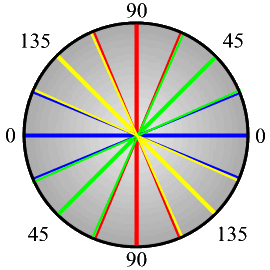
\includegraphics[width=5cm]{CannyEdgeWheel.png}\\
	\caption[Canny-Winkel]{Canny-Winkel}
	\label{fig:nettop}
\end{figure}

Dadurch sind alle "Arten" von Kanten abgedeckt: horizontal, vertikal und 2 mal diagonal. Die Richtung der Kante ist egal, deswegen kommt man mit 4 Möglichkeiten aus statt 8. Die Winkel werden  in 0, 45, 90 \& 135 Grad unterteilt.

Danach wird ein Threshold angewendet, um zu schwache Kanten auszufiltern und ein sauberes Bild zu generieren. Allerdings sind die meisten Kanten jetzt noch relativ dick, um damit zu arbeiten sollten sie aber jeweils 1 Pixel breit sein. Dafür gibt es mehrere Ansätze, wir haben uns für die Non-Max Suppression entschieden.\\
Hier wird abhängig von dem Winkel der Kante in der Umgebung nach Kanten gesucht und stärkste von ihnen ausgewählt. Sie bleibt im Bild, während die anderen, schwächeren Kanten entfernt werden. Konkret heißt das, dass bei einer horizontalen Kante in der vertikalen Umgebung nach stärkeren Kanten gesucht wird - sozusagen nach parallelen Kanten. Die Suchumgebung ist immer der Winkel der Kante um 90 Grad gedreht. \cite{canny1}


\subsection{Hough Transformation für Kreise}
Zur Erkennung der Kreisförmigen Spielsteine im entzerrtem Kantenbild kommt eine Hough-Transformation für Kreise zum Einsatz. \\
\\
Die Kreis-Hough-Transformation ist ein übliches Verfahren zum Erkennen von Kreisen und deren Mittelpunkte. Das Verfahren benötigt zur Erkennung eines Kreises mit dem Radius \(c\) ein Set an Kantenpunkten, die auf dem gesuchten Kreis liegen. \cite{houghnote2}\\
In einem zweidimensionalen Raum kann ein Kreis mithilfe von \\
\begin{equation}
(x - a)^2 +(y - b)^2 = c^2 
\end{equation} 
beschrieben werden. \cite{houghnote1} Wobei der Punkt \((x,y) \) ein Kantenpunkt auf dem Kreis ist, \((a,b)\) der Kreismittelpunkt und \(c\) der Radius des Kreises.\\

Liegt ein Punkt \((x,y)\) auf einem Kreis im Eingabebild und ist der Radius \(c\) bekannt so k\"onnen alle potenziellen Kreismittelpunkte \((a,b)\) mithilfe der oben erwähnten Formel ermittelt werden. Die Potenziellen Kreismittelpunkte werden in einem Akkumulator-Array gespeichert. Die Maxima in diesem Array repräsentieren die gefunden Kreismittelpunkte.\cite{houghnote2} Siehe Abbildung \ref{fig:hough2d}.\\

\begin{figure}[ht]
	\centering
		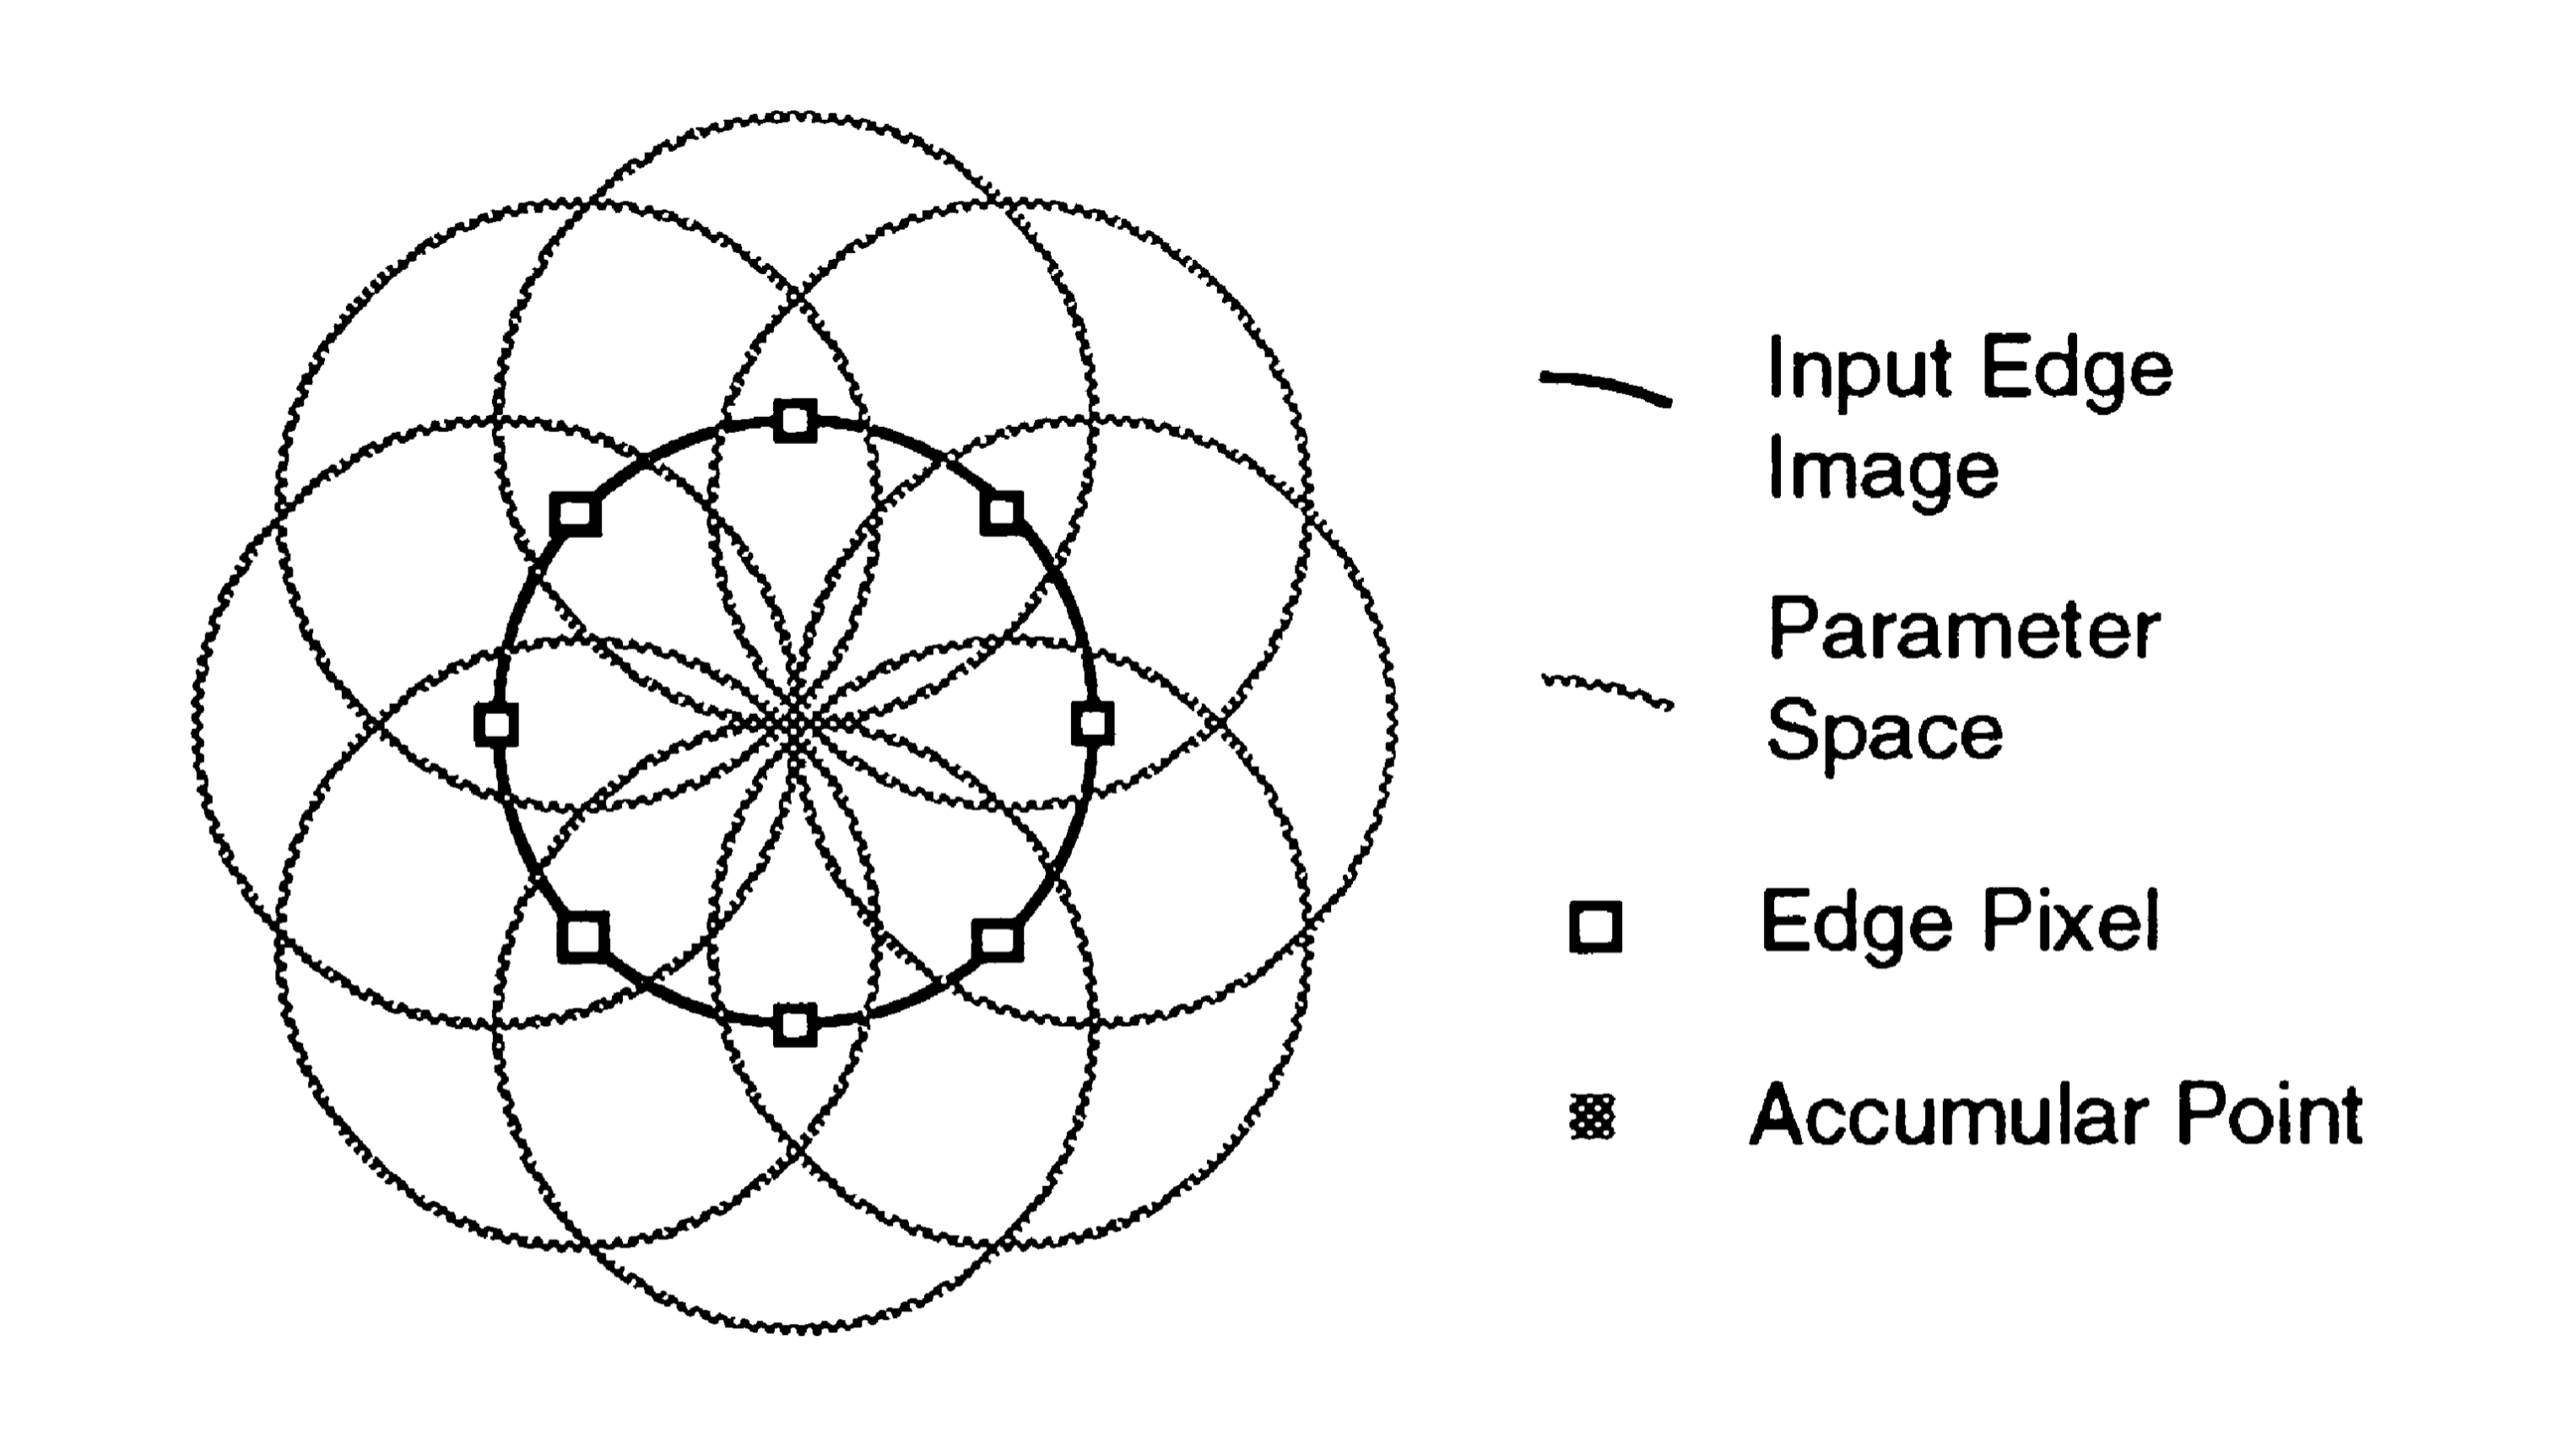
\includegraphics[width=6cm]{2dhough_darstellung.png}\\
	\caption[Funktion von Hough bei bekanntem Radius]{Funktion von Hough bei bekanntem Radius\cite{houghnote2}}
	\label{fig:hough2d}
\end{figure}

Wenn ein Punkt \((a,b,c)\) im Hough-Raum ein Maximum ist, so gibt es im Eingabebild einen Kreis mit dem Mittelpunkt \((a,b)\) und dem Radius  \(c\).
Visualisiert man die potenziellen Kreismittelpunkte des Kantenpunktes im dreidimensionalen Hough Raum, so werden diese als gerader Kreiskegel dargestellt.\cite{houghnote1}\\ Der Schnittpunkt \((a,b,c)\) von Maximal vielen Zylindern repräsentiert den gefundenen Kreismittelpunkt \((a,b)\) mit dem Radius \( c\).

\subsection{Gültigkeit des Spielzuges}
Zur Erkennung der Gültigkeit eines Spielzuges werden die Daten des Spielfelds vor und nach dem Zug verglichen. Falls ein unterschied erkannt wird, welcher in einem Zug nicht möglich wäre, wird die Nummer des Zuges sowie die Daten des Spielfelds vor und nach dem Zug ausgegeben. Somit kann überprüft werden ob es sich in dem Zug tatsächlich um einen ungültigen Spielzug handelt, oder ob ein Stein nicht richtig erkannt wurde.
Der Algorithmus wird ab dem 2. geladenen Bild nach jedem Bild einmal aufgerufen um die Korrektheit des jetzigen Zuges zu überprüfen.


\subsection{Farberkennung}
Die Farberkennung muss zwischen annähernd Weiß und Schwarz unterscheiden müssen. \\
Es reicht das entzerrte Bild als Grauwertbild auszulesen. Die Pixel der Kreismittelpunkte
werden mit 4 umliegend gemittelt und anschließend mit einem Schwellwert verglichen.\\
Grauwerte unter 80 stufen wir als Schwarz ein, über 50 als Weiß.

\subsection{Spielfeldpositionserkennung}
Die Position an der sich ein Stein befindet wird ermittelt, indem die erkannten Kreismittelpunkte
mit den zuvor gespeicherten Koodinaten der Spielfeldpsitionen verglichen werden.\\
Dafür werden die Distanzen zu allen Positionen ermittelt, 
wenn die Distanz kleiner ist als ein Schwellert,  wird er an dieser Position erkannt und gespeichert.
%%------------------------------------------------------

%%------------------------------------------------------
\section{Implementierung}
Die Implementierungspipeline sieht so aus, dass zuerst die Eckpunkte des Spielfelds mittels  einem Threshold erkannt werden. Die Eckpunkte werden dann verwendet, um das Spielfeld wieder zu einem perfekten Quadrat zu entzerren. Die Kanten des entzerrten Spielfelds werden mithilfe eines Canny Filters erkannt. Dabei sind nur die Kanten der Spielsteine wichtig, da diese bei der Kreiserkennung verwendet werden. Der nächste Schritt ist, die Anwendung einer Hough Kreiserkennung auf das Canny Kantenbild, um die Position der Spielsteine zu ermitteln. Danach werden mit einer eigens endwickelten Methode die Spielsteine auf ein virtuelles, aus einem 3 x 3 x 3 Array bestehendes, Spielfeld gelegt. Der letzte Schritt ist der Vergleich von zwei Zügen (Bildern) und das Entscheiden, ob dieser Zug gültig war. Dieser Schritt wird ebenfalls mit einem eigens entwickelten Algorithmus gelöst.

\subsection{Framework}
Das Framework ist so aufgebaut, dass alle 6 Methoden in einer Datei hintereinander, in einer for-Schleife, aufgerufen werden. Die Schleife läuft alle Bilder eines Spiels ab, wobei es egal ist, aus wie vielen Zügen ein Spiel besteht. Jede Methode liest jeweils ein Bild ein, verarbeitet dieses und speichert zum Schluss das verarbeitete Bild wieder ab.\\
In der Datei „main.m“ kann der User die Variable „game“ in Zeile 2 auf einen positiven Integer ändern, um auszuwählen welches Spiel analysiert werden soll. Ein weiterer Parameter, der vom User verändert werden kann, ist der Threshold, ebenfalls in der Datei „main.m“. Das Verändern der Variable „threshold“ auf einen Wert zwischen 0 und 1 verändert die Stärke des Thresholds.\\
Um das Programm zu starten, muss der User lediglich die Datei „main.m“ in Matlab ausführen. Standardmäßig wird das erste Spiel im Datensatz komplett analysiert. Das Ergebnis wird in der Konsole ausgegeben. Dort kann der User sehen, ob und wann unerlaubte Spielzüge auftreten.\\

\subsection{Threshold und Eckenerkennung}
Diese Methode liest RGB Bilder ein und gibt die 4 Eckpunkte des Spielfelds zurück. Außerdem wird das threshold Bild abgespeichert.\\
Als ersten Schritt wird das eingelesen Bild mittels der Matlab Methode „rgb2gray“ in ein Graustufenbild umgewandelt. Danach wird das Graustufenbild in ein Binärbild, mit der Methode „imbinarize“ und dem vom User definiertem threshold Wert, umgewandelt. Das Anwenden dieser 2 Methoden hintereinander hat bei unseren Tests bessere Ergebnisse erzielt als das alleinige Anwenden der Methode „imbinarize“. Um das Bild etwas zu säubern wird es anschließend mit einem  4 Pixel breitem kubischen Strukturelement erodiert. Das Ergebnis ist ein Binärbild in dem das Spielbrett weiß ist und der Hintergrund schwarz.\\
Mithilfe des Binärbildes können die Eckpunkte ermittelt werden. Es wird die Methode „find“ in Kombination mit „min“ und „max“ verwendet, um jeweils das erste und letzte weiße Pixel in einer Reihe und Spalte zu finden. Die roten Striche in dem nachfolgenden Bild sind jeweils auf Höhe des ersten weißen Pixels in +x, -x, +y und -y Richtung. Mithilfe von „min“ und „max“ können bei Koordinate der 4 Eckpunkte errechnet werden. Diese werden in einem Array abgespeichert und zurückgegeben.\\

\begin{figure}[ht]
	\centering
		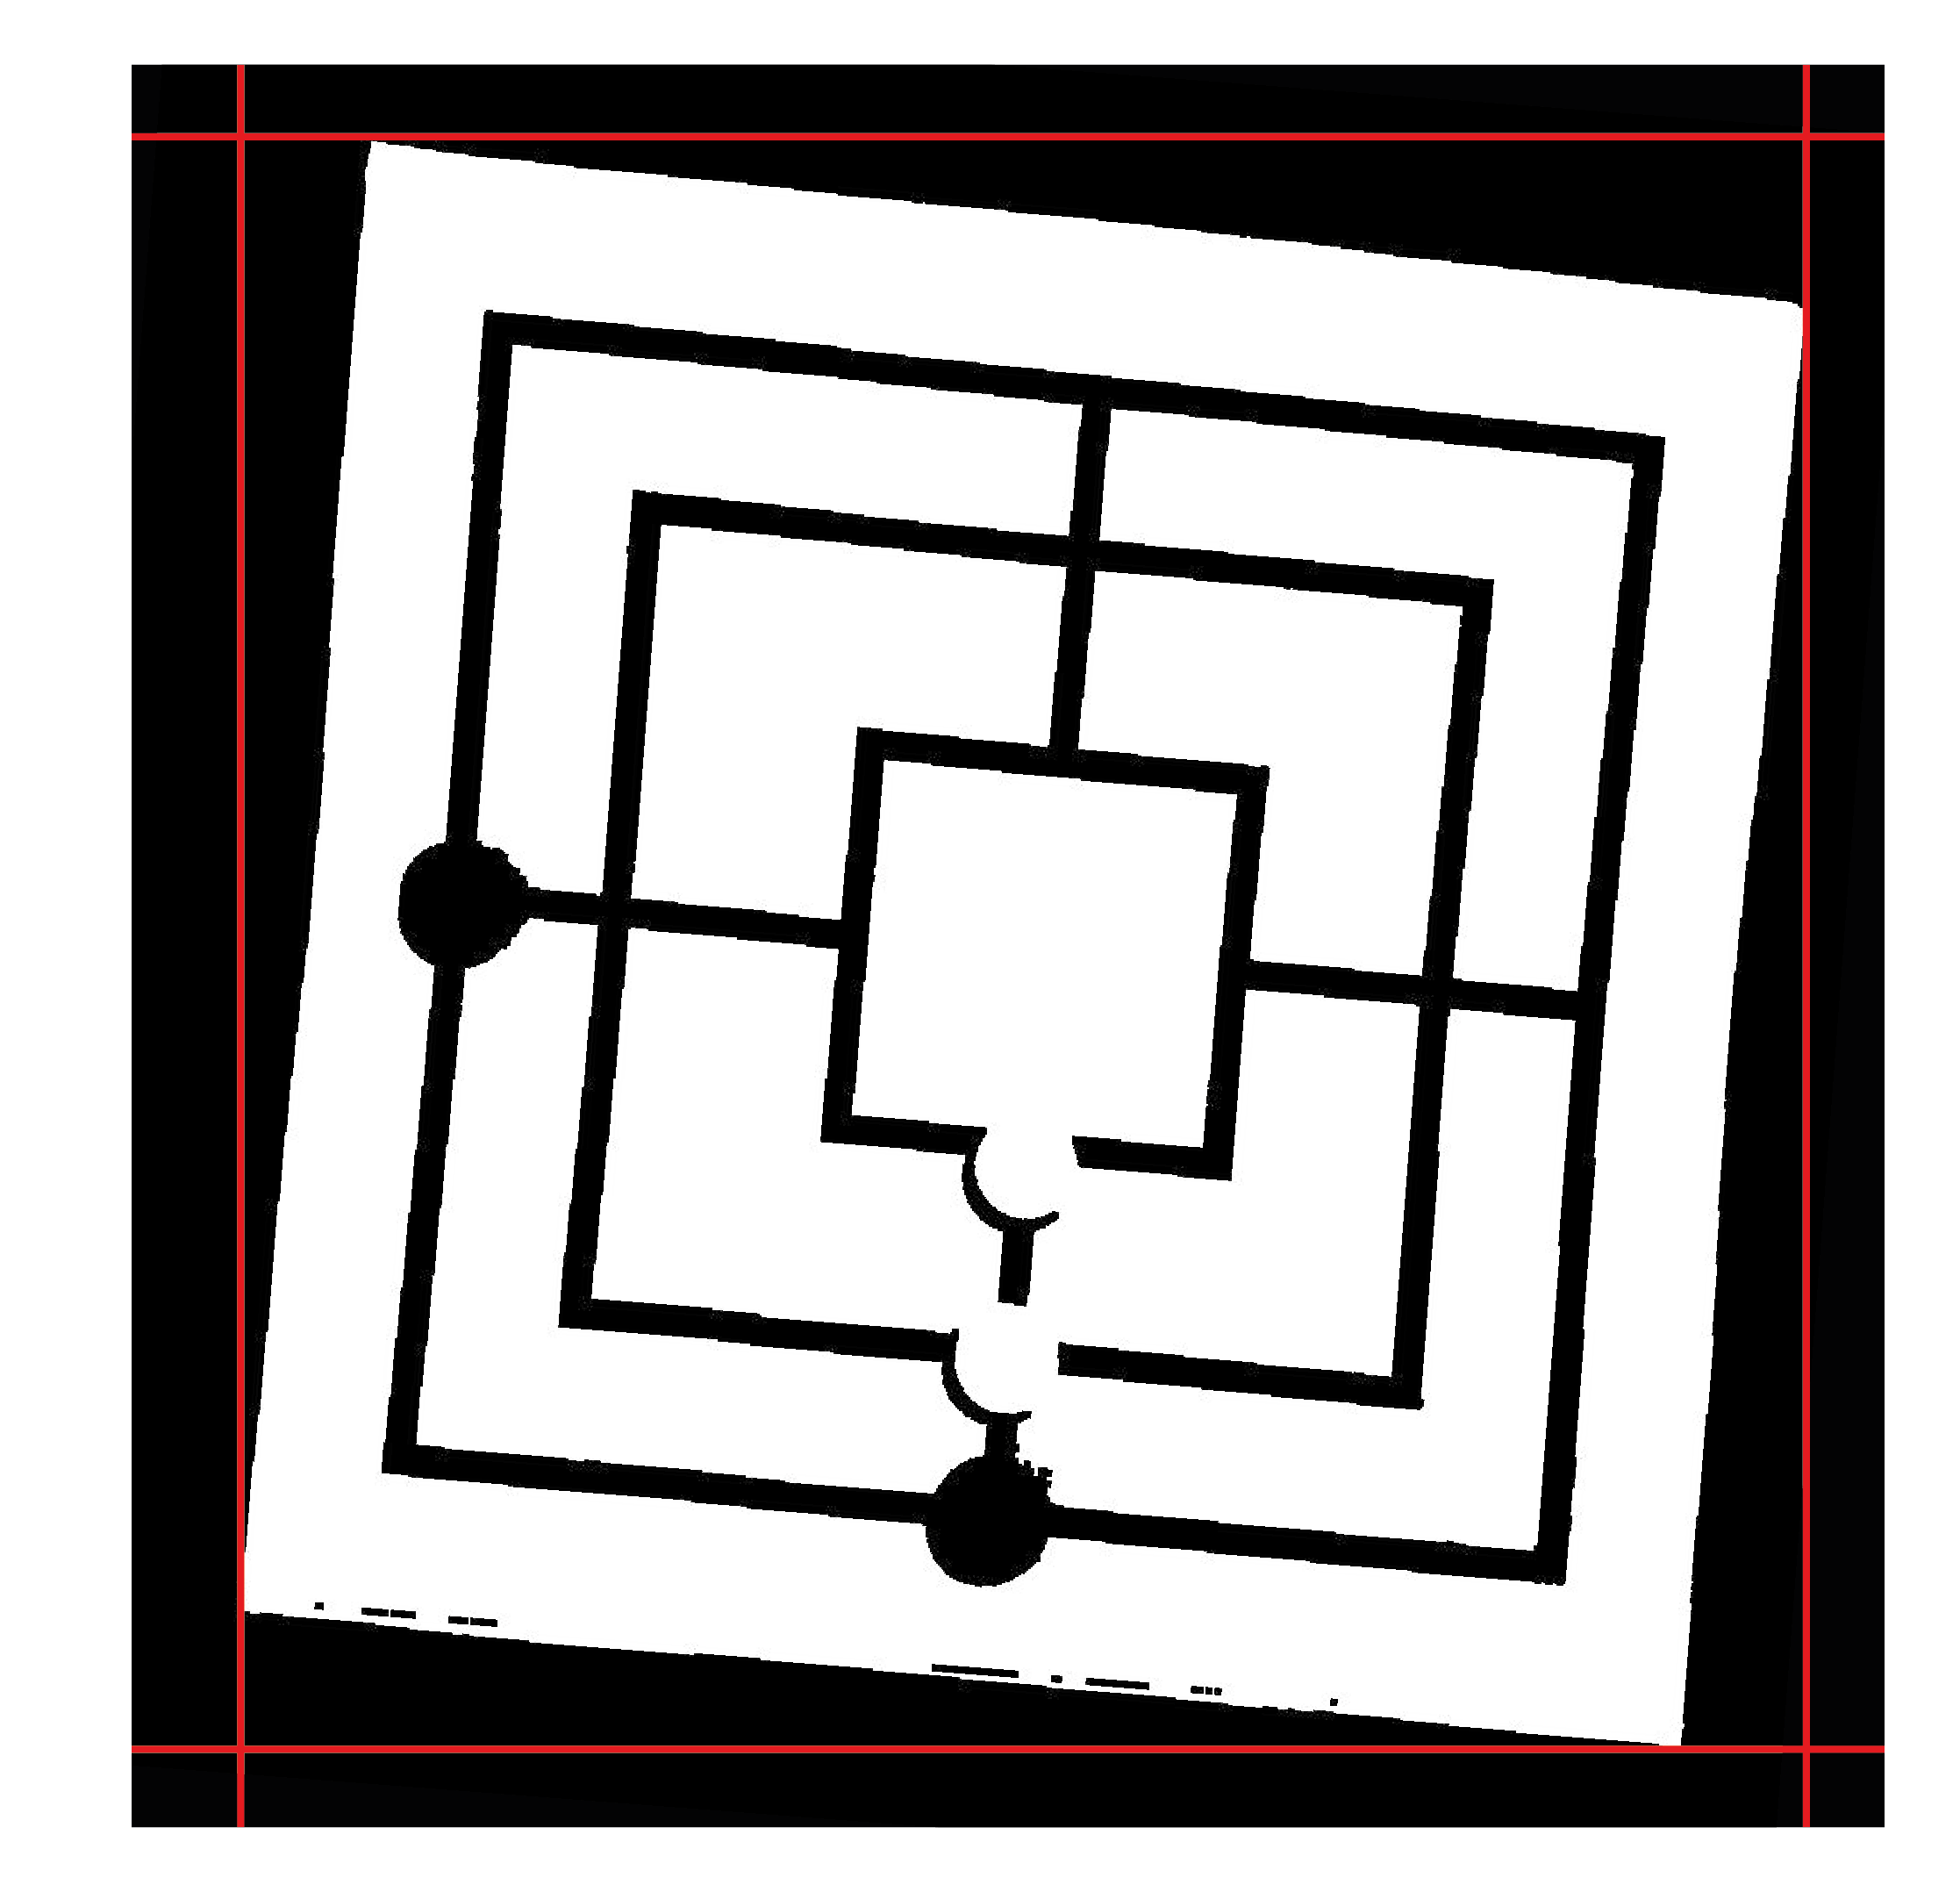
\includegraphics[width=8cm]{Ecken.png}\\
	\caption[Eckenerkennung]{Eckenerkennung}
	\label{fig:nettop}
\end{figure}

\subsection{Geometrische Transformation}
Diese Methode liest das originale RGB Bild ein und bekommt die 4 Eckpunkte übergeben. Das Ergebnis ist ein 500 x 500 Pixel RGB Bild mit dem entzerrten Spielfeld, wie man es an dem nachfolgenden Bild sehen kann.\\

\begin{figure}[ht]
	\centering
		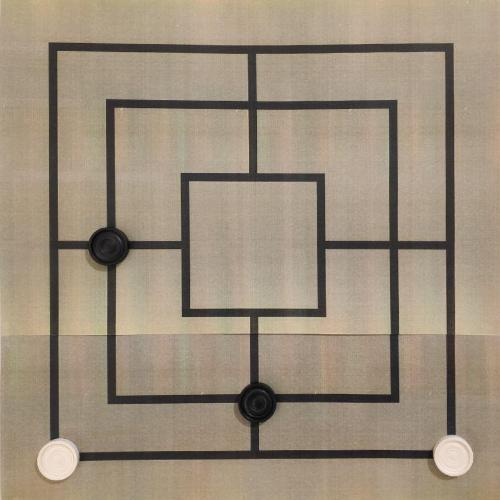
\includegraphics[width=6cm]{Spielbrett_Entzerrt.png}\\
	\caption[Spielfeld entzerrt]{Spielfeld entzerrt}
	\label{fig:nettop}
\end{figure}

Geometrische Transformation ist der Überbegriff für viele verschiedene Anwendungen. In diesem Fall ist aber das entzerren eins perspektivischen Quadrates gemeint. Dazu werden die Eckpunkte des verzerrten Quadrates und die Größe des Quadrates in entzerrter Form benötigt. Nach dem Entzerren wird ein 500 x 500 Pixel Quadrat ausgeschnitten und abgespeichert.\\
Zuerst muss die Transformationmatrix errechnet werden. Diese wird dann auf das verzerrte Bild angewendet, um dieses zu entzerren. Das Ergebnis ist ein Bild, in dem die 4 vorher definierten Punkte ein perfektes Quadrat bilden.\\
Die Koordinaten der jeweiligen Pixel ändern sich von Weltkoordinaten in Intrinsische Koordinaten nach der Transformation. Damit man das entzerrte Quadrat an den Eckpunkten ausschneiden kann, müssen die Eckpunkte zuerst in Intrinsische Koordinaten umgewandelt werden. Die Methode „imcrop“ mit den umgewandelten Koordinaten wird verwendet, um das Quadrat auszuschneiden. Das Ergebnis wird Abgespeichert.\\

\subsection{Canny Kantenerkennung}
Diese Methode liest ein entzerrte 500 x 500 Pixel RGB Bild ein und Speichert das dazugehörige Kantenbild ab.\\
Die Kantenerkennung nach Canny besteht aus einer Reihe von Schritten oftmals beginnend mit dem Anwenden eines Gauß’schen Weichzeichners auf das gesamte Bild. Weil das Spielfeld sehr klare Linien und Formen hat würde ein Weichzeichner das Ergebnis kaum verbessern, deshalb wird dieser Schritt in dieser Implementierung ausgelassen.\\
Der erste Schritt ist das Errechnen der Kantenkraft (wird für spätere Schritte benötigt), auch Magnitude genannt, indem man den Verlauf des Bildes mithilfe einer Sobel Matrix ausrechnet. Dieser Schritt muss jeweils in x- und y-Richtung durchgeführt werden.\\ 

\begin{figure}[ht]
	\centering
		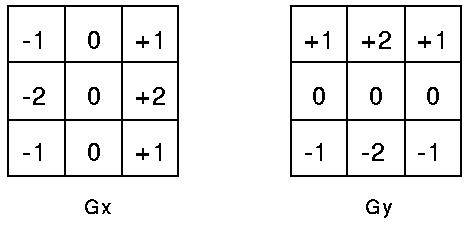
\includegraphics[width=8cm]{Sobel.png}\\
	\caption[Sobel Matrix]{Sobel Matrix}
	\label{fig:nettop}
\end{figure}

Die Länge der Hypotenuse der beiden Ankatheten Gx und Gy ist gleichzeitig auch die Magnitude.\\
Der nächste Schritt ist das Thresholding. Bei diesem Schritt werden Kantenpixel mit einem schwachen Magnitude Wert ausgefiltert. Das Ergebnis ist ein Kantenbild das nur starke Kanten enthält.\\
Der Letzte Schritt ist das Thinning, bei dem die Dicke der erkannten Kanten auf ein Pixel reduziert wird. Dies wird durch Non-Maximum-Supression erreicht. Dabei wird abhängig von dem Winkel der Kante in der Umgebung nach weiteren Kanten gesucht, um anschließend die "stärkste" Kante auszuwählen. Die schwächeren Kanten werden dann gelöscht, wodurch die Dicke auf 1 Pixel reduziert wird.\\

\subsection{Hough Kreiserkennung}
Die Funktion \(hough\) findet die Kreismittelpunkte von Kreisen mit einem Radius \(r\), \(radiusMin \leq r \leq radiusMax \)  und gibt diese als \(n * 2\) Matrix zurück. 
Um die Kreismittelpunkte zu finden liest die Funktion das Kantenbild des aktuellen Spieles und Spielzuges ein. \\
\\
Die Funktion \(hough\) ruft für alle ganzzahliegen Radien (\(radiusMin \leq r \leq radiusMax\)) die Funktion hufffixedRadius auf und speichert alle gefundenen Mittelpunkte, unabhängig des Radiuses, in einer einzigen Matrix. Der Radius wird nicht gespeichert da er für nächsten Schritte irrelevant ist.\\
\\
In der Funktion \(HoughFixedRadius\) wird über jedes Pixel des Kantenbildes iteriert. Falls das Pixel den Wert 1 hat, also ein Kantenpixel ist, werden m  viele potenzielle Kreismittelpunkte \((hy, hx)\)  abgeschlagen. Diese Punkte berechnen sich durch:  
\begin{equation}
x_{h} = x + radius * cos(t)
\end{equation}
\begin{equation}
y_{h} = y + radius *  sin(t).
\end{equation}
Wobei \(t = (2\pi/m)*i\) ist. 
Im zweidimensionalen Hough-Raum wird an der Stelle \((y_{h}, x_{h})\) der Wert um eins erhöht. Siehe Abbildung \ref{fig:houghfixed}.\\

\begin{figure}[ht]
	\centering
		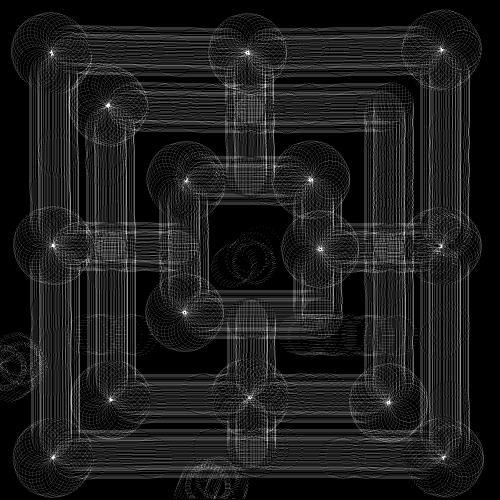
\includegraphics[width=8cm]{Huffexample3_16.jpg}\\
	\caption[Hough-Raum bei Radius = 20px]{Hough-Raum bei Radius = 20px}
	\label{fig:houghfixed}
\end{figure}

Anschließend wird das Array auf Maxima untersucht. Da mehrere Kreise gefunden werden müssen, ist es nicht ausreichend das Array auf das Feld mit dem maximalen Wert zu bestimmen. Deshalb wird vom User der Wert \(minHoughValue\) gesetzt (zwischen 0 und 1). Umso niedriger dieser Wert ist, umso mehr Kreise werden gefunden. Es steigt jedoch auch die Fehleranfälligkeit. Ist der Wert \(minHoughValue = 0\) so wird jedes Feld im Hough-Raum als Kreismittelpunkt gedeutet deren Wert \(\geq 0\) ist. Ist \(minHoughValue = 1\) so werden nur jene Felder als Kreismittelpunkte aufgefasst deren Wert \(\geq amountCenterPoints\) ist.  Falls ein Feld im Hough-Raum als Kreismittelpunkt aufgefasst wird, wird diese Position in einem Array gespeichert. \\
\\
Falls der Wert amountCenterPoints niedrieg gewählt wurde oder das eingelesene Kantenbild teilweise fehlerhaft ist. So kann es passieren das mehrer (leicht unterschiedliche) Kreismittelpunkte für den selben Kreis gefunden werden. Da nur die Mittelpunkte der Spielsteine relevant sind, wir davon ausgehen das alle Spielsteine annähernd gleich groß sind und dass nie zwei Spielsteine übereinander liegen, können alle gefundenen Kreismittelpunkte \((y_{j}, x_{j})\) deren Distanze zum Kreismittelpunkt \((y_{i}, x_{i})\) kleiner als der \(Radius\) ist gelöscht werden. \\
\\
Außerdem müssen wir beim Eingabebild voraussetzen, dass kein runder Gegenstand am Spielfeld liegt dessen Radius \(r\)  \(radiusMin \leq r \leq radiusMax\) ist. 
Anschließend gibt die Funktion HoughFixedRadius alle gefundenen Kreismittelpunkte für den vorgegeben Radius zurück. \\

Da handelsübliche Mühlesteine aus konzentrischen Kreisen aufgebaut sind, kann es passieren, dass für einen Spielstein der selbe Mittelpunkt für unterschiedliche Radien gefunden wird.  Da wir wie oben erwähnt davon ausgehen dass nie zwei Steine übereinander liegen, werden wieder alle doppelt gefundenen Mittelpunkte gelöscht. Mittelpunkte werden als Doppelt angesehen, wenn die Distanz zwischen zwei Mittelpunkten kleiner als der kleinstmögliche Radius ist. \\

Anschließend wird ein .jpg Bild, auf dem die Kreismittelpunkte weiß Makiert sind, sowie ein .txt file mit den Koordinaten der gefundenen Kreismittelpunkte auf dem Eingabebild gespeichert. Die Funktion Hough gibt die Kreismittelpunte als Matrix zurück. \\ 

\begin{figure}[ht]
	\centering
		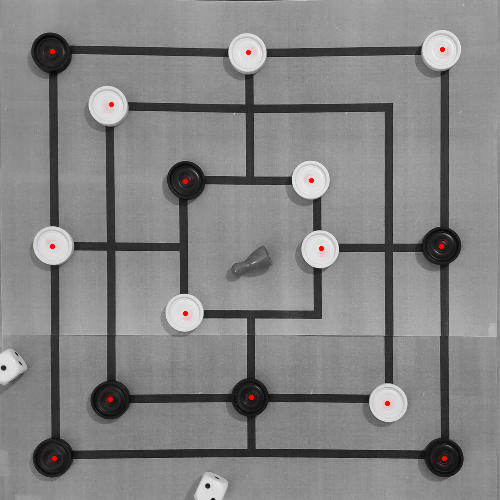
\includegraphics[width=8cm]{hough_performance.jpg}\\
	\caption[Gefundenen Kreismittelpunkte (rot) über dem entzerrten Graustuffenbild des Spielfeldes]{Gefundenen Kreismittelpunkte (rot) über dem entzerrten Graustuffenbild des Spielfeldes}
	\label{fig:hougresult}
\end{figure}


\subsection{Farberkennung und Spielfeldposition}
Diese Methode nimmt als Eingabeparameter, die bereits von Hough Funktion gefundenen Kreismittelpunkte. Sie vergleicht diese mit den Positionen an denen Mühlesteine platziert werden können.\\
Wenn sich ein gefundener Mittelpunkt nahe an einer Spielfeldposition, an der Steine abgelet werden können,  befindet,  wird die besetzte Position in einem Array markiert. \\
Um die Farbe des Steins zu erkennen, wird der Grauwert an der Stelle des von Hough gefundenen Mittelpunkt und vier weiteren umliegenden Punkten verglichen. Zum Vergleich dient ein Schwellwert. Die Farben werden  im Array als 1 oder 2 markiert und dann in eine 3x3x3 Matrix, die den Spielfelddimensionen entspricht eingetragen.\\
Diese Matrix wird dann als txt gespeichert und von der Funktion ausgegeben.

\subsection{Gültigkeit des Spielzuges}
Die Funktion „isLegit.m“ bekommt die Daten von einem Spielfeld vor und nach einem Zug, sowie die Nummer des Zuges übergeben. Zusätzlich speichert sie sich die Anzahl der Steine vor und nach dem Zug.
Falls sich die Anzahl der Steine um mehr als 1 unterscheidet handelt es sich bereits um einen ungültigen Zug. Daraufhin wird überprüft in welcher Phase sich das Spiel befindet (Platzierungsphase/Spielphase).\\
Das wird mittels der Funktion „getPhase.m“ gemacht. Die Funktion vergleicht zwei Spielfelder und findet heraus in welcher Spielphase sich das Spiel befinden müsste, damit es sich um einen legitimen Zug handelt. Es wird sich wieder die Anzahl der Steine gemerkt, jedoch muss man diesmal auch überprüfen ob eine neue Mühle geschlossen wurde, da sich so die Differenz der Anzahl der Steine anders verhält.\\
Hier wird die Funktion „checkForMill.m“ einmal pro Spielbrett (=2 mal) aufgerufen. „checkForMill.m“ wird ein Spielfeld übergeben und liefert zurück ob sich eine Mühle auf dem Spielfeld befindet. Es wird überprüft ob zumindest einer der zwei Spieler mehr als 2 Steine am Feld hat, und überprüft dann in jedem Ring des Spielfeldes im Uhrzeigersinn ob eine Mühle darauf liegt. Im äußersten Ring wird bei den belegten Eckpunkten analysiert ob in den zwei folgenden Feldern ebenfalls die selbe Farbe liegt, und bei den belegten Mittelpunkten wird überprüft ob eine Mühle die in die tiefe geht (= über alle 3 Ringe) existiert. Bei den inneren zwei Kreisen werden lediglich die Eckpunkte überprüft, da die Mittelpunkte bereits mit dem äußeren Ring gedeckt wurden.\\
Die Anzahl der schwarzen und weißen Steine wird über „countOccurences.m“ errechnet, welche ein Spielfeld übergeben bekommt und einen Vektor mit der Anzahl an Steinen pro Spieler zurückliefert.


%%------------------------------------------------------

%%------------------------------------------------------
\section{Evaluierung}

\subsection{Datensatz}
Anzahl der Bilder: 101
Größe der Bilder: 2000 x 2667 Pixel
Quelle des Datensatzes: selbst aufgenommen, Smartphonekamera, regelmäßge Ausleuchtung, keine harten Schatten, einfärbiger Hintergrund.\\

\subsection{Evaluierungsfragen}

\textbf{1. Wird das Spielfeld richtig eingelesen?} \\
Beim Spiel 1 wurden von 450 Spielsteinen, 2 Spielsteine nicht richtig erkannt. Ein Schwarzer und ein Weißer. Das ist eine Fehlerquote von 0.4 \%. \\
\\
Beim Spiel 2 wurden von 472 Spielsteinen 17 Spielsteine nicht richtig erkannt. Das ist eine Fehlerquote von 3 \%. Hier handelt es sich nur um Schwarze Spielsteine, die im oberen Bereich des Spielfeldes Platziert wurde. Hier werden zwar die Mittelpunkte der Kreise korrekt erkannt, jedoch können die steine nicht eindeutig einer Farbe zugeordnet werden. Das liegt an den starken Reflexionen auf den Spielsteinen liegen. \\ 
\\
Der Grund warum die Spielsteine im Game 1 schlechter erkannt wurden als im Game 2 liegt nicht an der Perspektive der Bilder, sondern an der veränderten Lichtsituation. Beim Spiel 2 wurde ein härteres und stärkeres Licht verwendet. \\
\\
Bei Game 3 wurden von 43 Spielsteinen 9 weiße Steine nicht richtig erkannt. Hier ist das Spielfeld weiß und aufgrund des geringen Kontrastes zu den Spielsteinen konnten die Kanten nicht richtig detektiert werden. Die schwarzen Spielsteine wurden allerdings ohne Fehler erkannt. \\
\\
Bei Game 4 handelt es sich um denselben Datensatz wie bei Game 3. Hier wurde allerdings der Kontrast im Nachhinein erhöht (Photoshop). Aufgrund dieser Bearbeitung wurden nur noch 5 weiße Steine nicht Korrekt erkannt. Das ist eine Quote von 11 \%.
\\

%Note: Game 1: 2 spielsteine nicht gefunden 1 Weißer 1 Schwarzer
%Game 2: Game 2: 17 Spielsteine. Aber immer 3 an der selben Position 
%Game 3: 9 weiße Steine wurden nicht erkannt. von 24
%Game 4: selber datensatz nur kontrast erhöht 5 steine nicht gefunden. 


%\textbf{2. Wird ein gültiger Spielzug vorhergesagt?}
\textbf{2. Wird ein gültiges Spiel als solches erkannt?}
\\

\textbf{Gültigkeit des Spielzuges}\\
Unter der Annahme, dass die Spielsteine auf den Beispielbildern richtig erkannt wurden, wird ein gültiges Spiel als solches erkannt. Da unsere Beispielbilder immer von einem ganzen Spiel sind ist es relativ leicht zu überprüfen in welcher Spielphase wir uns befinden. Deswegen wird angenommen dass die Bilder mit dem ersten Zug anfangen.\\
Wäre dies nicht der Fall, müsste man sich über den Unterschied der Spielsteine errechnen in welcher Spielphase man sich gerade befindet. Jedoch geht das nur unter der Annahme, dass die Daten von einem von einem gültigen Zug stammen. Das würde jedoch den ganzen Algorithmus redundant machen.\\
Immer wen ein Spiel als nicht gültig erkannt wird, werden die zwei 3x3x3 Matrizen ausgegeben damit diese mit den Eingabebildern verglichen werden können.


\subsection{Evaluierung der Funktionen}
\textbf{Threshold}\\
Die Eckenerkennung mithilfe eines Threshold funktioniert nur wenn der Kontrast zwischen Spielfeld und Hintergrund hoch genug ist. Idealerweise sollte der Hintergrund einfärbig sein. Ist der Hintergrund nicht einfärbig oder gibt es Blendenflecken bzw. Spiegelungen wird das Spielfeld höchstwahrscheinlich nicht richtig erkannt.  Blendenflecken sind besonders problematisch da sie weiß sind und als Ecken missinterpretiert werden könnten.\\
\\
\textbf{Geometrische Transformation}\\
Solange 4 Eckpunkte im vorherigen Schritt erkannt werden kann kein Fehler bei der Geometrische Transformation auftreten. Werden falsche Eckpunkte erkannt, wird das Spielfeld zwar falsch verzerrt, aber das Programm läuft weiter. Die richtige Erkennung der Eckpunkte wird vorausgesetzt damit das Programm korrekt läuft.\\
\\
\textbf{Canny}\\
Die Kantenerkennung funktioniert sehr gut bei unserem Spielfeld. Da das Spielfeld aus klaren Linien und Formen besteht, gibt es kaum Problemen bei der Erkennung. Ein Korrektes Katenbild ist für die Erkennung der Spielsteine wichtig. Es müssen lediglich die Kanten der Spielsteine erkannt werden damit das Programm richtig laugt. Aufgrund dessen kann die Position der Spielsteine auch richtig erkannt werden, wenn sich Fremdgegenstände auf dem Spielfeld befinden. \\
\\
\textbf{Hough Kreiserkennung}\\
Die Performance der Kreiserkennung hängt sehr stark mit der Qualität des übergebenen Kantenbild ab. Bei guten Kantenbilder wie bei Game 1 und 2 werden die Kreismittelpunkte mit einer geringen Toleranz immer richtig erkannt. Hier kann es lediglich passieren das der gefundene Kreismittelpunkt des Spielsteines um wenige Pixel vom tatsächlichen Kreismittelpunkt des Spielsteines abweicht. Das ist wahrscheinlich darauf zurück zu führen das die Kantenbilder in relativ geringer Auflösung übergeben werden.\\
\\
Bei den Bildern der Spielen 3 und 4 kann die Funktion öfters keine Kreise detektieren. Die schlechtere Performance bei diesem Teil des Datensatz ist darauf zurückzuführen, dass die weißen Spielsteine nur kaum oder garnicht auf dem übergebenen Kantenbild zu erkennen sind. Also das lediglich ein bruchteil der Kreislinie vorhanden ist. \\
\\
\textbf{Farberkennung und Spielfeldposition} \\
Hier wurde die Position der übergebenen Kreismittelpunkte mit den Ecken den möglichen Positionen verglichen. Desweiteren wurde untersucht ob es sich um einen schwarzen oder weißen Spielstein handelt. \\
Die erkennung der Position funktion korrekt solange die Dimensionen des Spielfeldes mit denen den in Absatz 1.4 beschriebenen Voraussetzungen übereinstimmen und alle Spielsteine annähernd korrekt positioniert sind. Für andere Spielfelder müssen die Koordinaten der möglichen Spielstein Positionen geändert werde. \\
\\
Die Erkennung der Farbe der Spielsteine funktioniert gut solange nicht ein zu hartes Licht verwendet wurde. Ansonsten können auf schwarzen Spielsteinen weiße Flecken auftreten, die falsch Interpretiert werden könnten. \\
\\
Bei den Spielen 1, 3 und 4 hat die erkennung der Spielsteine korrekt funktioniert. Lediglich beim Spiel 2 sind Fehler bei den schwarzen Spielsteinen aufgetreten. \\
\\





%%------------------------------------------------------

%%------------------------------------------------------
\section{Schlusswort}
Das Ergebnis unseres Projektes ist ein lauffähiges Matlab-Projekt, das Bilder von Mühle-Spielen, die den den spezifizierten Vorbedingungen entsprechen, auslesen und erkennen kann, ob der getätigte Spielzug gültig ist. Die Ausgabe erfolgt über .txt Dateien.
Insgesamt sind wir zufrieden mit unserer Arbeit. Anfangs gab es etwas Verwirrung über die Pipeline, mit hilfe unseres Tutors wurde die aber beseitigt.
%Mit unseren Vorbedingungen lassen sich die Bilder gut auslesen, natürlich könnte man diese weiter verkleinern, indem man an den Algorithmen feilt.\\
\\
Die erkennung der Spielsteine hat unter bedingunge wie in den Voraussetzungen beschrieben, sehr gut Funktioniert. Lediglich weniger als 1 \% der Spielsteine wurde nicht korrekt erkannt (Spiel 1). Bei etwas schlechterem Bildmaterial konnte wir allerdings noch immer mehr als 95\% der Spielsteine korrekt erkennen. \\
\\
Eine mögliche verbesserung wäre eine GUI mit der man das Spielfeld und die Farbwerte der Eingabebilder kalibrieren kann. Dadurch wäre es möglich das Programm auf unterschiedlichen Spielfeldern zu erkennen. \\
\\



%%------------------------------------------------------


%%------------------------------------------------------
\bibliographystyle{plain}
\bibliography{edbv_lit}
%%Bei verwendung von Latex schreibt ihr eure Referenzen in ein eigenes bib-File (siehe hier edbv_lit.bib). Jene Referenzen, die ihr im Bericht mittels \cite zitiert, werden automatisch in die Referenzliste übernommen. Weitere Information zum Einbinden von BibTex gibt es hier: http://www.bibtex.org/Using/de/
%%------------------------------------------------------


\end{document}
\grid
\grid
